\documentclass[12pt,a4paper]{article}
\usepackage{amsmath,amscd,amsbsy,amssymb,latexsym,url,bm,amsthm}
\usepackage{epsfig,graphicx,subfigure}
\usepackage{enumitem,balance}
\usepackage{wrapfig}
\usepackage{mathrsfs,euscript}
\usepackage[usenames]{xcolor}
\usepackage{hyperref}
\usepackage[vlined,ruled,linesnumbered]{algorithm2e}
\usepackage{array}
\hypersetup{colorlinks=true,linkcolor=black}

\newtheorem{theorem}{Theorem}
\newtheorem{lemma}[theorem]{Lemma}
\newtheorem{proposition}[theorem]{Proposition}
\newtheorem{corollary}[theorem]{Corollary}
\newtheorem{exercise}{Exercise}
\newtheorem*{solution}{Solution}
\newtheorem{definition}{Definition}
\theoremstyle{definition}

\renewcommand{\thefootnote}{\fnsymbol{footnote}}

\newcommand{\postscript}[2]
 {\setlength{\epsfxsize}{#2\hsize}
  \centerline{\epsfbox{#1}}}

\renewcommand{\baselinestretch}{1.0}

\setlength{\oddsidemargin}{-0.365in}
\setlength{\evensidemargin}{-0.365in}
\setlength{\topmargin}{-0.3in}
\setlength{\headheight}{0in}
\setlength{\headsep}{0in}
\setlength{\textheight}{10.1in}
\setlength{\textwidth}{7in}
\makeatletter \renewenvironment{proof}[1][Proof] {\par\pushQED{\qed}\normalfont\topsep6\p@\@plus6\p@\relax\trivlist\item[\hskip\labelsep\bfseries#1\@addpunct{.}]\ignorespaces}{\popQED\endtrivlist\@endpefalse} \makeatother
\makeatletter
\renewenvironment{solution}[1][Solution] {\par\pushQED{\qed}\normalfont\topsep6\p@\@plus6\p@\relax\trivlist\item[\hskip\labelsep\bfseries#1\@addpunct{.}]\ignorespaces}{\popQED\endtrivlist\@endpefalse} \makeatother

\usepackage{tikz}
\usepackage{multicol}
\usepackage{tcolorbox}
\tcbuselibrary{skins}
\tcbsubskin{mycross}{empty}{frame code={%
    \draw[line width=1pt] (frame.south west)--(frame.north east);
    \draw[line width=1pt] (frame.north west)--(frame.south east);},
    skin first=mycross,skin middle=mycross,skin last=mycross 
}
\usepackage{float}

\begin{document}
\noindent

%========================================================================
\noindent\framebox[\linewidth]{\shortstack[c]{
\Large{\textbf{Lab07-Amortized Analysis}}\vspace{1mm}\\
CS214-Algorithm and Complexity, Xiaofeng Gao \& Lei Wang, Spring 2021.}}
\begin{center}
\footnotesize{\color{red}$*$ If there is any problem, please contact TA Yihao Xie. }

\footnotesize{\color{blue}$*$ Name: Log Creative  \quad Student ID:  \quad Email: logcreative-lzl@sjtu.edu.cn}
\end{center}
\begin{enumerate}
	\item Suppose we perform a sequence of $n$ operations on a data structure in which the $i$ th operation costs $i$ if $i$ is an exact power of 2, and 1 otherwise. Use an accounting method to determine the amortized cost per operation.
	
	\begin{solution}
		% For the $i$-th operation, an amortized cost $\hat{C}_i=\$3$ is charged.
		% \begin{itemize}
		% 	\item \$1 pays for itself.
		% 	\item \$2 is stored for later cost expansion, \$1 for paying one of the recent $\frac{i}{2}$ items, \$1 for paying one of the old $\frac{i}{2}$ items.
		% \end{itemize}
		Define $C_i$ as the cost of the $i$th operation,
		\begin{equation*}
			C_i=\left\{\begin{aligned}
				&i, &&\text{if }i\text{ is an exact power of 2},\\
				&1, &&\text{otherwise}
			\end{aligned}\right.
		\end{equation*}
		\begin{description}
			\item[Case 1: $i$ is not the power of 2.] an amortized cost $\hat{C_i}=\$3$ is charged:
			\begin{itemize}
				\item \$1 pays for itself;
				\item \$2 is stored for later cost expanding, \$1 \$1 for paying one of the recent $\frac{i}{2}$ items, \$1 for paying one of the old $\frac{i}{2}$ items.
			\end{itemize} 
			\item[Case 2: $i$ is the power of 2.]  an amortized cost $\hat{C_i}=\$2$ is charged, in order not to have leftouts.

		\end{description}

		\begin{figure}[h]
			\centering
			\begin{tikzpicture}[node distance=0.5cm]
\tikzstyle{arr}=[minimum width=0.5cm,draw];
\node[arr] (v1) at (-2,1.5) {1};
\node [arr] (v2) at (-1.5,1.5) {2};
\node [arr] (v3) at (-1,1.5) {3};
\node [arr] (v4) at (-0.5,1.5) {4};
\node [arr] (v5) at (0,1.5) {5};
\node [arr] (v6) at (0.5,1.5) {6};
\node [arr] (v7) at (1,1.5) {7};
\node [arr] (v8) at (1.5,1.5) {8};
\node [above of=v1] {\$0};
\node [above of=v2] {\$0};
\node [above of=v3] {\$0};
\node [above of=v4] {\$0};
\node [above of=v5] {\$2};
\node [above of=v6] {\$2};
\node [above of=v7] {\$2};
\node [above of=v8,node distance=1cm] {\$2};

\node[arr] (v1) at (4.5,1.5) {1};
\node [arr] (v2) at (5,1.5) {2};
\node [arr] (v3) at (5.5,1.5) {3};
\node [arr] (v4) at (6,1.5) {4};
\node [arr] (v5) at (6.5,1.5) {5};
\node [arr] (v6) at (7,1.5) {6};
\node [arr] (v7) at (7.5,1.5) {7};
\node [arr] (v8) at (8,1.5) {8};
\node [above of=v1] {\$0};
\node [above of=v2] {\$0};
\node [above of=v3] {\$0};
\node [above of=v4] {\$0};
\node [above of=v5] {\$0};
\node [above of=v6] {\$0};
\node [above of=v7] {\$0};
\node [above of=v8] {\$0};

\node at (3,1.5) {$\rightarrow$};
\end{tikzpicture}
		\end{figure}
	
		Thus,
		\begin{equation*}
			T(n) = \sum_{i=1}^n C_i \leq \sum_{i=1}^n \hat{C_i} = 3n - \lfloor \log_2 n \rfloor
		\end{equation*}
	\end{solution}

	\item Consider an ordinary \textbf{binary min-heap} data structure with $n$ elements supporting the instructions \textsc{Insert} and \textsc{Extract-Min} in $O(\log n)$ worst-case time. Give a potential function $\Phi$ such that the amortized cost of \textsc{Insert} is $O(\log n)$ and the amortized cost of \textsc{Extract-Min} is $O(1)$, and show that it works.
	
	% Extract-min find and delete min
	
	\begin{solution}
		Let $\Phi$ be the sum of the cost on every node
		\begin{equation*}
			\Phi(S_i) = \sum_{k=1}^i \log_2 k
		\end{equation*}
		
		which meets the requirement of a potential function:
		\begin{equation*}
			\Phi(S_n) \geq \Phi(S_0) = 0
		\end{equation*}
		because it has to be the nonnegative integer.

		Describe \textsc{Insert} and \textsc{Extract-Min} for binary min-heap data as follows:
		\begin{multicols}{2}
			\textsc{Insert}
			\begin{enumerate}
				\item Insert the element to the end of the heap.
				\item \textsc{Perlocate-Up} from the insertion position.
			\end{enumerate}

			
			\textsc{Extract-Min}
			\begin{enumerate}
				\item Extract the minimum element.
				\item Put the last element to the root.
				\item \textsc{Perlocate-Down} from root.
			\end{enumerate}
		\end{multicols}
		
		Because both \textsc{Perlocate-Up} and \textsc{Perlocate-Down} take $\log_2 n = O(\log n)$, so both the algorithms cost $C_i = O(\log n)$.

		As for the amortized analysis, the potential function is considered:
		% \begin{multicols}{2}
		\textsc{Insert} The number of element will be increased by 1.

		\begin{align*}
			\hat{C_i} &= C_i + \Phi_i - \Phi_{i-1}\\
					&= 1 + \log_2 i + \log_2 i = 2\log_2 i + 1
		\end{align*}

		\textsc{Extract-Min} The number of element will be decreased by 1.

		\begin{align*}
			\hat{C_i} &= C_i + \Phi_i - \Phi_{i+1} = 2 + \log_2 i - \log_2 (i+1) = 2 + \log_2 \frac{i}{i+1} < 2
		\end{align*}

		So the amortized cost for \textsc{Insert} is $O(\log n)$ and for \textsc{Extract-Min} is $O(1)$.

		% \begin{description}
		% 	\item[Case 1: new layer is introduced.] 
			
		% 	\input{img/insertnew.tex}

			
		% 	\item[Case 2: no new layer is introduced.] 
			
		% 	\begin{tikzpicture}
\tikzstyle{tnode}=[circle,draw,minimum width=0.5cm];
\tikzstyle{dnode}=[tnode,fill=gray];

\node [tnode] (v1) at (0,2) {};
\node [tnode] (v2) at (-1,1) {};
\node [tnode] (v5) at (1,1) {};
\node [tnode] (v3) at (-1.5,0) {};
\node [tnode] (v4) at (-0.5,0) {};
\node [tnode] (v6) at (0.5,0) {};
\node [dnode] (v7) at (1.5,0) {};
\draw  (v1) edge (v2);
\draw  (v2) edge (v3);
\draw  (v2) edge (v4);
\draw  (v1) edge (v5);
\draw  (v5) edge (v6);
\draw  (v5) edge (v7);
\end{tikzpicture}
			
		% 	\begin{align*}
		% 		\hat{C_i} &= C_i + \Phi_i - \Phi_{i-1}\\
		% 				&= 1 + \log_2 i
		% 	\end{align*} 
		% \end{description}
		% So the amortized cost of \textsc{Insert} is $O(\log n)$.

		% \textsc{Extract-Min}
		% \begin{description}
		% 	\item[Case 1: a layer is removed.] Then, the potential after the removal
		% \end{description}
		% \end{multicols}
		
	\end{solution}

	\item Assume we have a set of arrays $A_0, A_1, A_2,\cdots$, where the $i^{th}$ array $A_i$ has a length of $2^i$. Whenever an element is inserted into the arrays, we always intend to insert it into $A_0$. If $A_0$ is full then we pop the element in $A_0$ off and insert it with the new element into $A_{1}$. (Thus, if $A_{i}$ is already full, we recursively pop all its members off and insert them with the elements popped from $A_0,...,A_{i-1}$ and the new element into $A_{i+1}$ until we find an empty array to store the elements.) An illustrative example is shown in Figure \ref{Fig-MultiArray}. Inserting or popping an element take $O(1)$ time.

	\begin{figure}[!htbp]
	\centering
	\includegraphics[width=0.5\textwidth]{Fig-MultiArray.pdf}
	\caption{An example of making room for one new element in the set of arrays.}
	\label{Fig-MultiArray}
	\end{figure}

    \begin{enumerate}
        \item In the worst case, how long does it take to add a new element into the set of arrays containing $n$ elements?
        \begin{solution}
			The worst case comes to that $n$ is the power of 2, assumming it to be $n=2^i$. All elements from $A_0, \cdots, A_{i-1}$ has to be popped and pushed into $A_i$, which is the last column. The inserted element will be inserted into $A_i$ as well.
			\begin{equation*}
				T(n) = 2(1+\cdots + 2^{i-1})+1 = 2^{i+1}-1 = 2n-1 = \Omega(n)
			\end{equation*}
		\end{solution}
        \item Prove that the amortized cost of adding an element is $O(\log n)$ by \emph{Aggregation Analysis}.
        \begin{solution}
			Enumerate the cost of different $n$:

			\begin{table}[h]
				\centering
				\begin{tabular}{l|cccccccc}
					\hline
					$i$ 			& 1 & 2 & 3 & 4 & 5 & 6 & 7 & 8 \\
					$C_i$(new push) 	& 1 & 1 & 1 & 1 & 1 & 1 & 1 & 1 \\
					$C_i$(pop+push)	&   & 2 &   & 6 &   & 2 &   & 14\\
					\hline
					$i$ 			& 9 & 10& 11& 12& 13& 14& 15& 16\\
					$C_i$(new push) 	& 1 & 1 & 1 & 1 & 1 & 1 & 1 & 1 \\
					$C_i$(pop+push)	&   & 2 &   & 6 &   & 2 &   & 30\\
					\hline
				\end{tabular}
			\end{table}

			Denote $S(n)$ as the sum of operations for inserting $n$ elements. The recurrence of $S(n)$ is:
			\begin{align*}
				S(1) &= 1\\
				S(2^i-1) &= 2S(2^{i-1}-1) + T(2^{i-1})\\
				S(2^i) &= S(2^{i}-1) + T(2^i)
			\end{align*}

			Because the worst case comes to $n=2^i$, the aggregation analysis will provide the upper bound reflected by the case of $\frac{S(2^i)}{2^i}$.

			\begin{align*}
				S(2^i) &= 2^{i+1}-1 + S(2^i-1) \\
					&= 2^{i+1} - 1 + 2S(2^{i-1}-1) + T(2^{i-1})\\
					&= 2^{i+1} - 1 + 2^{i-1}S(1) + 2^{i-2}T(2^1) + \cdots + 2^1T(2^{i-2}) +T(2^{i-1})\\
					&= 2^{i+1} - 1 + 2^{i-1} + 2^i - 2^{i-2} + 2^i - 2^{i-3} + \cdots + 2^i - 1\\
					&= 2^{i+1} +(i-1)2^i
			\end{align*}

			By \emph{Aggregation Analysis}, the amortized cost of adding an element is
			\begin{equation*}
				\hat{C_i} =\frac{S(n)}{n}=\frac{S(2^i)}{2^i} = i+1 = \log_2 n + 1 = O(\log n)
			\end{equation*}
		\end{solution}
        \item If each array $A_i$ is required to be sorted but elements in different arrays have no relationship with each other, how long does it take in the worst case to search an element in the arrays containing $n$ elements? 
    
		\begin{solution}
			Binary Search in each $A_i$.
			\begin{equation*}
				T(n) = 1+2+\cdots+\log(n+1)-1 = \frac{1}{2}\log(n+1)(\log(n+1)-1) = O(\log^2 n)
			\end{equation*}
			\begin{tcolorbox}[skin=mycross]
			If the array is sorted, then the search algorithm is as follows:
			\begin{algorithm}[H]
				\caption{The searching algorithm for sorted arrays}
				\KwIn{set of arrays $A_0,A_1,\cdots, A_i$, the element $x$ to be searched}
				\KwOut{the searching result}
				\BlankLine
				\For(){$j\leftarrow 0$ to $i$}{
					\If(){$A_j$ is not empty and (head of $A_j) \leq x \leq$ (tail of $A_j$)}{
						\ForEach(){$y$ in $A_j$}{
							\lIf(){$x=y$}{
								\Return{$(j,$ position of $y$ in $A_j)$}
							}
						}
					}
				}
				\Return{No such an element is found}\;
			\end{algorithm}

			In the worst case, the element is in the last array to be searched and near the tail of the array. And the element is in the range of every array. In other word, the number of elements satisfies
			\begin{equation*}
				n = 2^0 + 2^1 + \cdots + 2^i = 2^{i+1}-1
			\end{equation*}
			the number of arrays satisfies
			\begin{equation*}
				i = \log_2 (n+1)-1
			\end{equation*}
			The time complexity comes to
			\begin{equation*}
				T^\prime(n) = 2i + n = 2(\log_2(n+1)-1) + n = \Omega(n)
			\end{equation*}
			
		\end{tcolorbox}
		\end{solution}

		\item What is the amortized cost of adding an element in the case of (c) if the comparison between two elements also takes $O(1)$ time?
		
		\begin{solution}
			% Now it becomes a little different, because the sorting algorithm has to be performed with a time complexity of $O(n\log n)$ \textbf{on every step}. The starting point of $A_0$ make every state to be sorted. On the base of the analysis in (b), now the amortized cost becomes

			% \begin{equation*}
			% 	\hat{C_i}^\prime = \hat{C_i} + O(n\log n) = n\log n + \log_2 n + 1 = O(n\log n)
			% \end{equation*}
			
			\begin{table}[H]
				\centering
				\begin{tabular}{l|cccccccc}
					\hline
					$i$ 			& 1 & 2 & 3 & 4 & 5 & 6 & 7 & 8 \\
					$C_i$(new push) 	& 1 & 1 & 1 & 1 & 1 & 1 & 1 & 1 \\
					$C_i$(pop+push)	&   & 2 &   & 6 &   & 2 &   & 14\\
					$C_i$(sort) 	& 	& $Q(3)$ & 	& $Q(7)$ &   & $Q(3)$ &   & $Q(15)$ \\
					\hline
					$i$ 			& 9 & 10& 11& 12& 13& 14& 15& 16\\
					$C_i$(new push) 	& 1 & 1 & 1 & 1 & 1 & 1 & 1 & 1 \\
					$C_i$(pop+push)	&   & 2 &   & 6 &   & 2 &   & 30\\
					$C_i$(sort)		& 	& $Q(3)$ & 	& $Q(7)$ & 	& $Q(3)$ & 	& $Q(31)$\\
					\hline
				\end{tabular}
			\end{table}


			Like Merge Sort. $O(\log n)$. Bit-Flip.

			\begin{tcolorbox}[skin=mycross]
			Enumerate the cost of different $n$ with sorting, where sorting requires $Q(n)=O(n\log n)$ time complexity:

			

			Because it starts from $A_0$, every pop will lead to a sort operation over the influnced elements. Let $S^\prime$ be the sum of new cost.

			\begin{align*}
				S^\prime(1) &= 1\\
				S^\prime(2^i-1) &= 2S^\prime(2^{i-1}-1) + T(2^{i-1}) + Q(T(2^{i-1}))\\
				S^\prime(2^i) &= S^\prime(2^{i}-1) + T(2^i)+ Q(T(2^i))
			\end{align*}

			By the same \emph{aggregation analysis} process, denote 
			\begin{equation*}
				R(n)=T(n)+Q(T(n))=2n-1+O((2n-1)\log(2n-1))
			\end{equation*}
			Then, in the worst case sum,
			\begin{align*}
				S^\prime(2^i) &= 
				% 2^{i+1}-1+ O((2^{i+1}-1)\log(2^{i+1}-1)) + S^\prime(2^i-1) \\
				% &= 2^{i+1}-1+ O((2^{i+1}-1)\log(2^{i+1}-1)) \\&+ 2^i - 1 + O((2^i-1)\log(2^i-1)) + 2S^\prime(2^{i-1}-1)
				2^{i+1} - 1 + 2^{i-1}S^\prime(1) + 2^{i-2}R(2^1) + \cdots + 2^1R(2^{i-2}) +R(2^{i-1})\\
				&= S(2^i) + \sum_{j=0}^{i-2} 2^j R(2^{i-1-j})\\
				&= S(2^i) + (2^i-1)\sum_{j=0}^{i-2} O(\log(2^{i-j}-1))\\
				&= S(2^i) + O\left((2^i-1)\frac{(i+2)(i-1)}{2}\right)
			\end{align*}
			So the new amortized cost is
			\begin{align*}
				\hat{C_i}^\prime = \frac{S^\prime(n)}{n}= \frac{S^\prime(2^i)}{2^i} &= \hat{C_i} +\frac{(2^i-1)O(i^2)}{2^i} \\&= O(\log n) + O((\log n)^2)\\&=O((\log n)^2)
			\end{align*}

		\end{tcolorbox}
		\end{solution}
    \end{enumerate}
	
\end{enumerate}



\textbf{Remark:} Please include your .pdf, .tex files for uploading with standard file names.


%========================================================================
\end{document}
